\documentclass[10pt,twocolumn,letterpaper]{article}

\usepackage{iccv}
\usepackage{times}
\usepackage{epsfig}
\usepackage{graphicx}
\usepackage{amsmath}
\usepackage{amssymb}

% Include other packages here, before hyperref.

% If you comment hyperref and then uncomment it, you should delete
% egpaper.aux before re-running latex.  (Or just hit 'q' on the first latex
% run, let it finish, and you should be clear).
\usepackage[pagebackref=true,breaklinks=true,letterpaper=true,colorlinks,bookmarks=false]{hyperref}

 \iccvfinalcopy % *** Uncomment this line for the final submission

% Pages are numbered in submission mode, and unnumbered in camera-ready
\ificcvfinal\pagestyle{empty}\fi

\begin{document}

%%%%%%%%% TITLE
\title{CAP 5516 Medical Image Computing Spring 2022 Project Proposal}

\author{Kyle Beggs\\
Department of Mechanical and Aerospace Engineering\\ 
University of Central Florida\\
{\tt\small kbeggs07@knights.ucf.edu}}

\maketitle
% Remove page # from the first page of camera-ready.
\ificcvfinal\thispagestyle{empty}\fi


\begin{abstract}
    1D models of the cardiovascular system are useful for surgical planning where time is of the essence due to their much reduced computational cost. These models are built form extracting the centerlines from 3D geometry. It is important for centerline extraction to not miss any branches as this can impact results and having a fully automated pipeline for simulation which includes centerline extraction is an attractive feature. State-of-the-art centerline extraction methods require user input and fail to capture branches often. This project seeks to further improve upon current approaches using Neural Networks for centerline extraction.
\end{abstract}


\section{Problem Definition}

In recent years there has been significant interest in developing a pipeline for cardiovascular surgical planning for patient-specific care via 3D Computational Fluid Dynamics (CFD) simulations \cite{morrisonAdvancingRegulatoryScience2018}. The main barrier to the implementation of such a tool for surgeons to use is computational cost, despite sustained advancements in compute power. However, the success of many proposed surgeries such as coronary bypasses depends on macro-hemodynamic quantities that can be accurately simulated with 1D models effectively reducing the computational cost by a factor of hundreds compared to 3D. An equally important goal in building a pipeline for patient-specific cardiovascular surgical planning is to be fully automated. Recent research thrust in this direction aims for these goals but requires user input \cite{pfallerAutomatedGeneration0D2021}.
 
Centerline extraction can be performed via the grassfire or shrinking ball algorithms with no user input, but these often fail to achieve the robustness needed for the results to be directly used in simulation. They often have unphysiologically small vessel branches near bifurcations and struggle where there might be sudden widening or narrowing of vessels, which is common in diseased patients. Other approaches simulate a wave front by solving the Eikonal equation or compute a minimum cost path, however, these require input of a seed and/or target outputs \cite{antigaCenterlineComputationGeometric2003} \cite{jinRobustEfficientCurve2016}.

In light of this, the goal of this project is to improve upon the current state of the art neural networks to segment the centerline of the vessel is desirable such that no user input is required and no further pre-processing is needed before performing 1D surgical planning simulations.


\section{Related Work}

The first attempt at extracting centerlines (at least claimed by the authors) was by Guo et al. who used a Fully Convolutional Network for extracting coronary artery centerlines \cite{guoDeepCenterlineMultitaskFully2019}. Lenga et al. built a system to extract centerlines on rib bones using the feature map output from the network to perform an external extraction algorithm \cite{lengaDeepLearningBased2019}. Although technically not using Deep Learning to output centerlines, it is included because it is fully-automated and that is a goal of this project. The next deep learning approach to extracting centerlines is DeepVesselNet where they attempt to segment the geometry, centerline, and bifurcation points \cite{tettehDeepVesselNetVesselSegmentation2020}. They use a cross-hair filter for speeding up computation and introduce a new loss function based on cross-entropy but takes into account the high class imbalance as centerlines represent a very small fraction (< 3\%) of the total pixels in an image. They also use angiogenesis models to generate synthetic data to train on since obtaining 3D vascular datasets along with centerline labels are nonexistent. The most recent attempt by Mostafa et al. first identifies a seed point and then narrows the input image to a CNN to the local area around that point. The output of the CNN is the next point on the centerline, which then becomes the new local area input into the CNN \cite{mostafaImprovedCenterlineExtraction2021} - similar to the wave front technique pioneered by Antiga et al.

\section{Technical Approach}

An approach similar to that of Guo et al. \cite{guoDeepCenterlineMultitaskFully2019} is used with ground truth labels representing the centerlines as 1-pixel wide `lines' and generated using a `baseline' method that is a current state of the art that is not a neural network. The input to the network is the segmentation and output is a centerline distance map and branch endpoints which are then fed into a minimal path graph algorithm to produce the final centerline. This approach is used because complex and well performing segmentation networks exists, and so we want to begin from that point. The method should also be generalizable as its approach to finding branch endpoints does not rely on detecting particular anatomical features as in \cite{mostafaImprovedCenterlineExtraction2021}. Endpoints are needed in the minimal path algorithm for final output of the centerline but represent a tiny fraction of the total voxels, suffering from major class imbalance. Guo et al. remedies this problem by generating a confidence map around the endpoint using a Gaussian distribution. This project attempts to make use of an `extreme' class imbalance loss function for detection of the endpoints from \cite{tettehDeepVesselNetVesselSegmentation2020} so further alleviate the problem.

\begin{figure}[t]
\begin{center}
   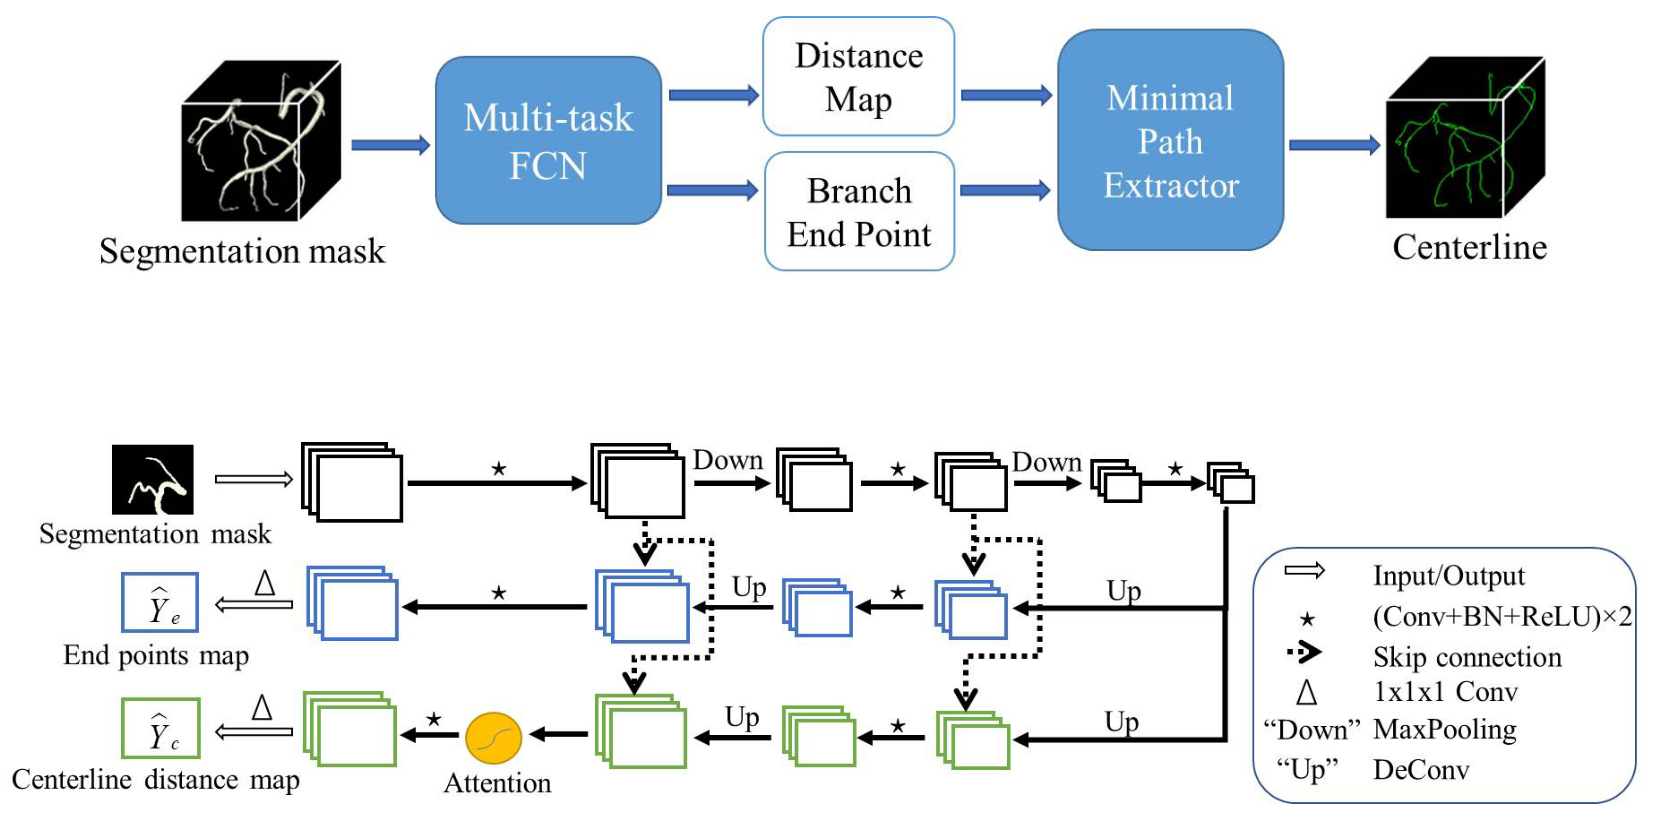
\includegraphics[width=0.8\linewidth]{network-arch-guo.png}
\end{center}
   \caption{Network architecture used by Guo et al. \cite{guoDeepCenterlineMultitaskFully2019} and the base for this work.}
\label{fig:fig1}
\end{figure}

\section{Experiments}

Two objectives will be investigated:
\begin{enumerate}
    \item Does the extreme class imbalance loss function developed in \cite{tettehDeepVesselNetVesselSegmentation2020} improve branch endpoint detection?
    \item What is the effect of training with perfect ground truth centerlines over truths generated with current state-of-the-art methods?
\end{enumerate}

Objective two is a continuation of a question posed at the conclusion of Guo et al. because they generated the truth centerlines using current state-of-the-art methods (termed `baseline') and then compared their network to those same baselines. Despite the conundrum of this approach, they still found their method was able to generalize better and increased accuracy of 30\%! They propose using the better output from their method to then train a second network and perhaps achieve even higher accuracies. Metrics that will be used to assess final performance: mean centerline to centerline distance, Hausdorff distance, and overall success rate which is defined determines that the centerline covers all branches sufficiently, has no spurious false positive branch, no wrong bifurcation, and no obvious deviation from the center throughout all sections.

Due to the lack of cardiovascular datasets freely available, the only two datasets found are used. A synthetic dataset from the DeepVesselNet paper and a real dataset from the Vascular Model Repository \cite{wilsonVascularModelRepository2013}. The DeepVesselNet synthetic dataset has 136 images and will be useful in testing the robustness of the network as it has a large amount of bifurcations and variance in vessel size. The Vascular Model Repository dataset contains 92 models and will be good for testing generalizability as it contains a spectrum of cardiovascular anatomy while the DeepVesselNet images look similar to each other.


%\begin{figure*}
%\begin{center}
%\fbox{\rule{0pt}{2in} \rule{.9\linewidth}{0pt}}
%%\includegraphics[width=0.8\linewidth]{figure2.pdf}
%\end{center}
%   \caption{Optional detailed illustration of your approach.}
%\label{fig:fig2}
%\end{figure*}

%\begin{table}
%\begin{center}
%\begin{tabular}{c c}
%\hline
%Method & Accuracy \\
%\hline
%Theirs & 0.5 \\
%Yours & 0.75\\
%Ours & \bf 0.9 \\
%\hline
%\end{tabular}
%\end{center}
%\caption{Results for your milestone and final reports.}
%\end{table}


{\small
\bibliography{centerline_bifurcation}
\bibliographystyle{IEEEtran}
}

\end{document}
